\clearpage

\section{Results}

In this section we provide the results of the inclusive and targeted searches. The observed and predicted \MET\ distributions for the
inclusive analysis are indicated in Fig.~\ref{fig:results_incl}. A summary of the results in the signal regions is provided in
Table~\ref{tab:results_incl}. In the low \MET\ region (\MET\ $<$ 100 GeV) which is dominated by the \zjets\ background, the observed
yields are in good agreement with the predicted background. This is also the case in the high \MET\ region (\MET\ $>$ 200 GeV).
In the moderate \MET\ region (100 $<$ \MET $<$ 200 GeV) we observe a slight excess in the data with respect to the predicted background.
Taking into account the full uncertainty on the background prediction, the significance of the excess is about 1.3$\sigma$. 
The separate results for the ee and $\mu\mu$ channels are presented in App.~\ref{app:results}. For this \MET\ region, we find an excess
of 1.4$\sigma$ in the ee channel and 0.7$\sigma$ in the $\mu\mu$ channel.


\begin{figure}[!h]
\begin{center}
\begin{tabular}{cc}
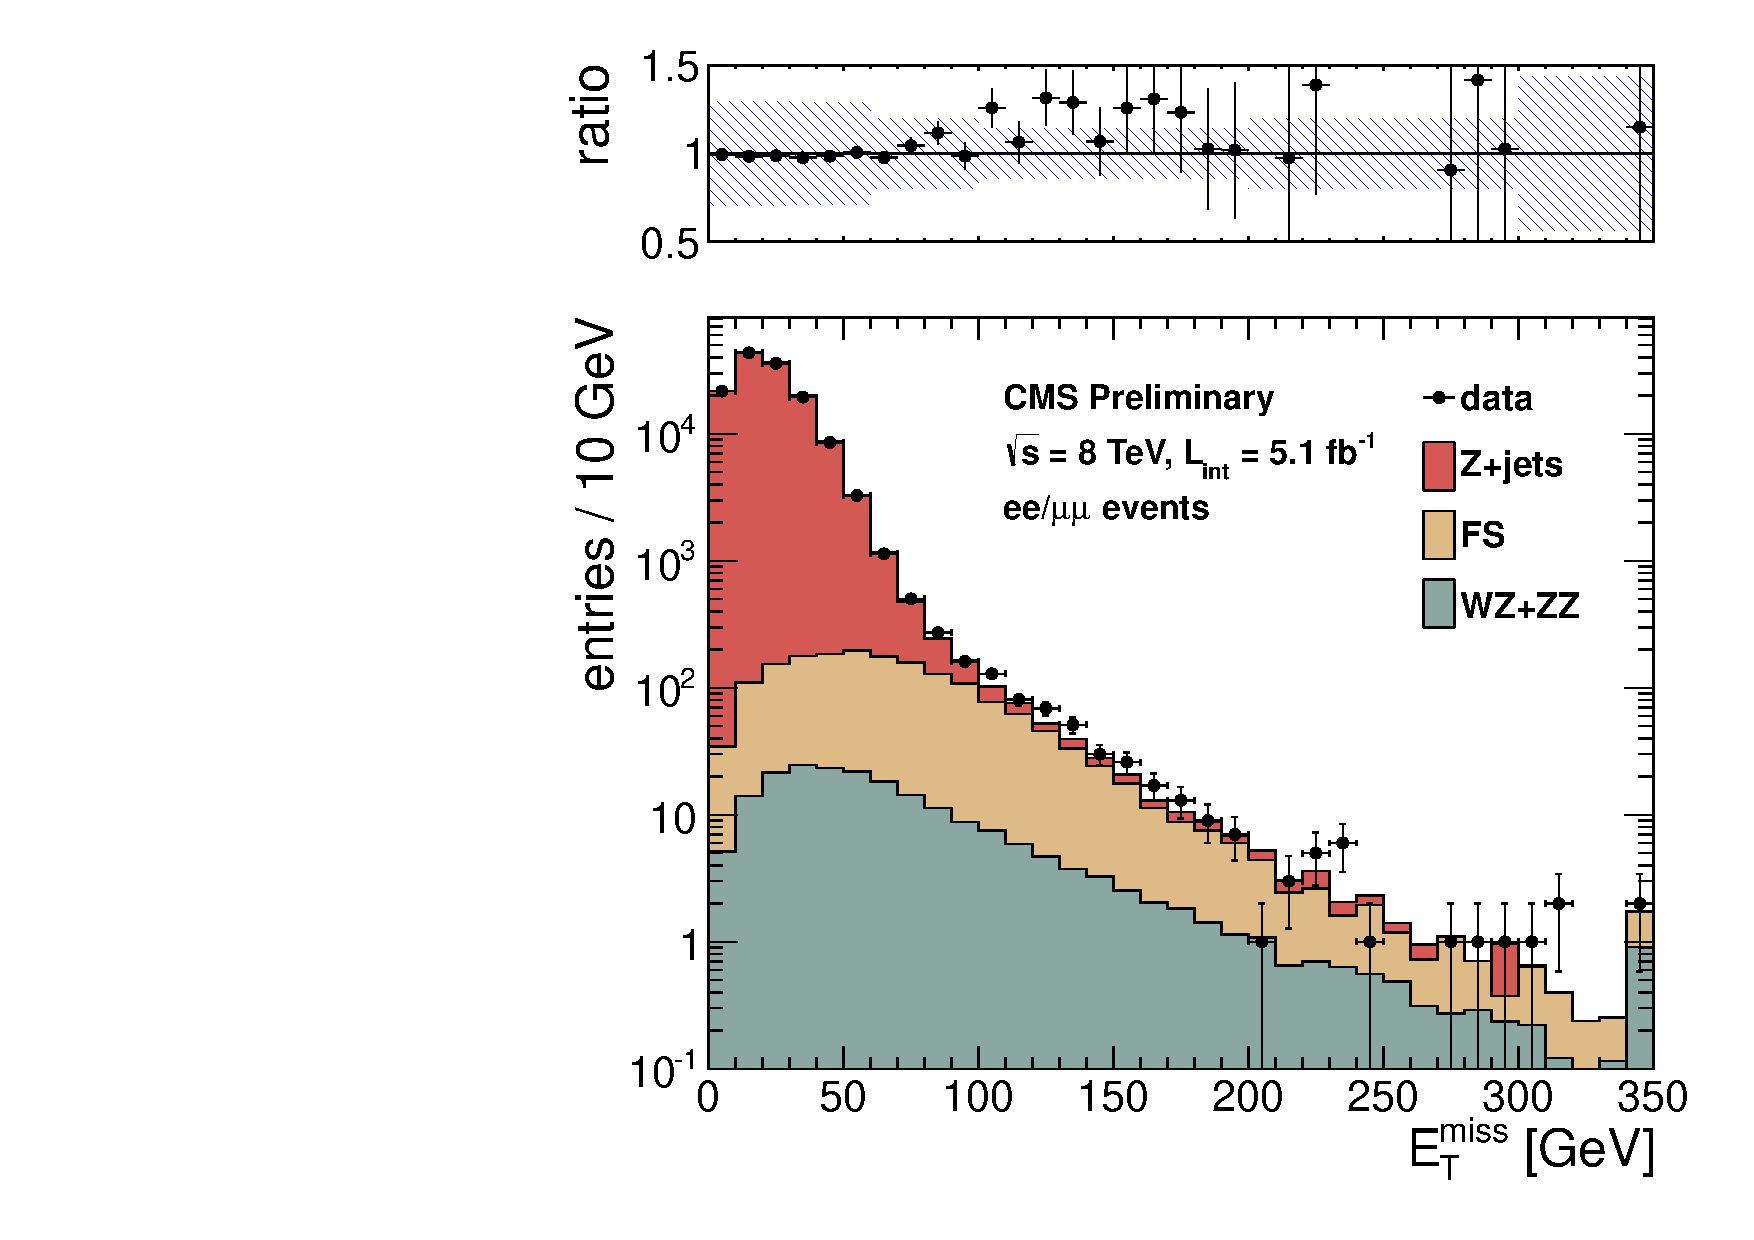
\includegraphics[width=0.6\textwidth]{plots/met_0.pdf}
\end{tabular}
\caption{Results of the inclusive analysis. The observed \MET\ distribution (black points) is compared with the sum of the predicted \MET\
distributions from \zjets, flavor-symmetric backgrounds, and WZ+ZZ backgrounds. The ratio of observed to predicted yields in each bin is
indicated. The error bars indicate the statistical uncertainty in the data and the shaded band indicates the total background uncertainty.
\label{fig:results_incl}
}
\end{center}
\end{figure}



\begin{table}[htb]
\begin{center}
\footnotesize
\caption{\label{tab:results_incl} Summary of results in the inclusive analysis. The total background is the sum of the \zjets\ background predicted from
the \MET\ templates method (\zjets\ bkg), the flavor-symmetric background predicted from e$\mu$ events (FS bkg), and the WZ and ZZ backgrounds predicted from MC
(WZ bkg and ZZ bkg). All uncertainties include both the statistical and systematic components. The Gaussian significance of the deviation between the data 
and total background is indicated for signal regions with at least 20 observed events. }
\begin{tabular}{l|c|c|c|c|c|c}

\hline
\hline
                      &   \MET\ $>$ 0 GeV   &  \MET\ $>$ 30 GeV   &  \MET\ $>$ 60 GeV   & \MET\ $>$ 100 GeV   & \MET\ $>$ 200 GeV   & \MET\ $>$ 300 GeV  \\
\hline
        \zjets\ bkg   &134792 $\pm$ 40438   &  32856 $\pm$ 9858   &    1546 $\pm$ 464   &   68.6 $\pm$ 20.8   &     4.3 $\pm$ 1.4   &     0.0 $\pm$ 0.0  \\
             FS bkg   &    1539 $\pm$ 239   &    1281 $\pm$ 199   &     793 $\pm$ 123   &      274 $\pm$ 43   &    13.7 $\pm$ 2.5   &     1.8 $\pm$ 1.1  \\
             WZ bkg   & 168.6 $\pm$ 134.9   & 132.5 $\pm$ 106.0   &   71.6 $\pm$ 57.3   &   28.9 $\pm$ 23.1   &     4.2 $\pm$ 3.4   &     0.9 $\pm$ 0.7  \\
             ZZ bkg   &   35.6 $\pm$ 28.5   &   31.1 $\pm$ 24.9   &   21.8 $\pm$ 17.5   &    11.9 $\pm$ 9.5   &     2.5 $\pm$ 2.0   &     0.6 $\pm$ 0.5  \\
\hline
          total bkg   &136535 $\pm$ 40439   &  34300 $\pm$ 9860   &    2432 $\pm$ 484   &      383 $\pm$ 54   &    24.7 $\pm$ 4.9   &     3.3 $\pm$ 1.4  \\
               data   &            134793   &             33810   &              2526   &               456   &                24   &                 5  \\
       significance   &              -0.0   &              -0.0   &               0.2   &               1.3   &              -0.1   &                    \\
\hline
\hline
\end{tabular}
\end{center}
\end{table}

\clearpage

The observed and predicted \MET\ distributions for the
targeted analysis are indicated in Fig.~\ref{fig:results_targ}. A summary of the results in the signal regions is provided in
Table~\ref{tab:results_targ}. The observed yields are in good agreement with the predicted background in all signal regions.

\begin{figure}[!h]
\begin{center}
\begin{tabular}{cc}
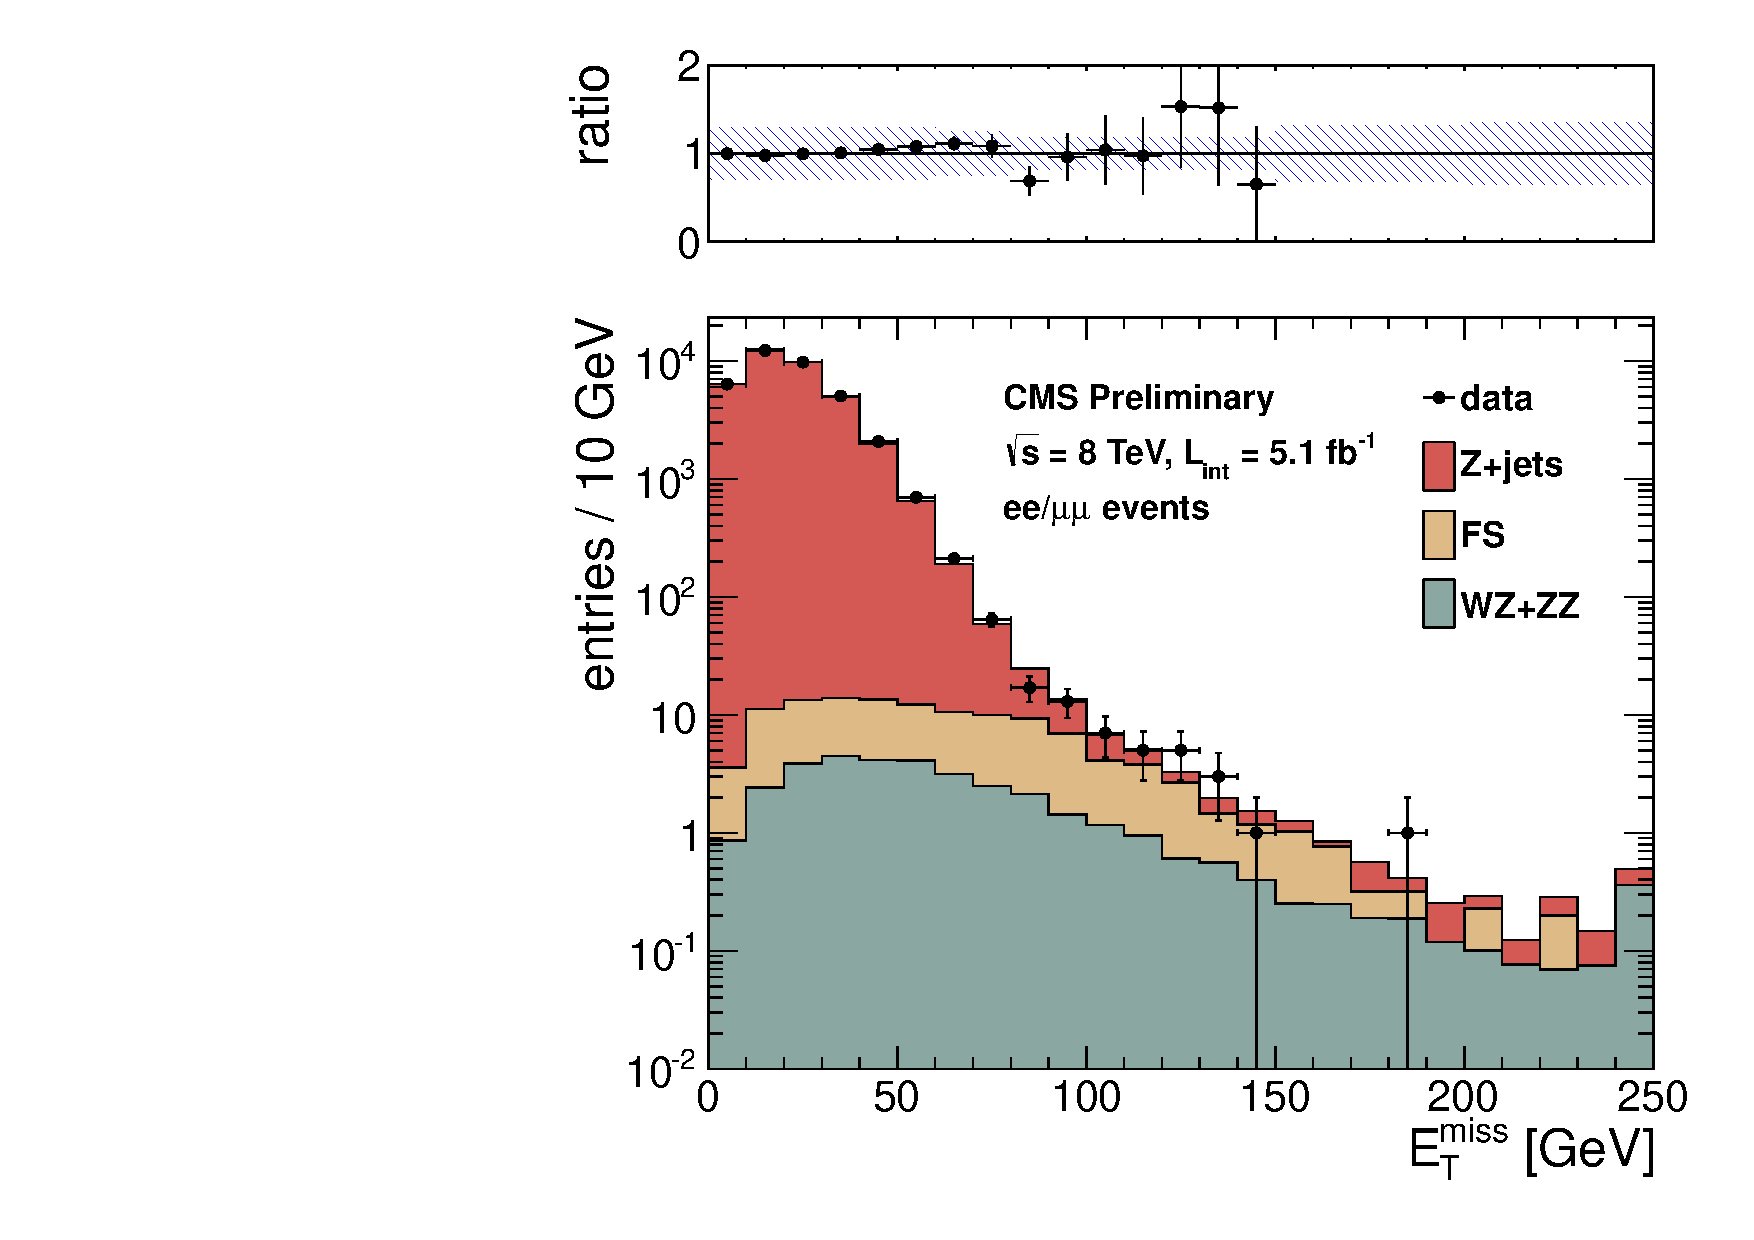
\includegraphics[width=0.6\textwidth]{plots/met_bveto_0.pdf}
\end{tabular}
\caption{Results of the targeted analysis. The observed \MET\ distribution (black points) is compared with the sum of the predicted \MET\
distributions from \zjets, flavor-symmetric backgrounds, and WZ+ZZ backgrounds. The ratio of observed to predicted yields in each bin is
indicated. The error bars indicate the statistical uncertainty in the data and the shaded band indicates the total background uncertainty.
\label{fig:results_targ}
}
\end{center}
\end{figure}



\begin{table}[htb]
\begin{center}
\scriptsize
\caption{\label{tab:results_targ} Summary of results in the targeted analysis. The total background is the sum of the \zjets\ background predicted from
the \MET\ templates method (\zjets\ bkg), the flavor-symmetric background predicted from e$\mu$ events (FS bkg), and the WZ and ZZ backgrounds predicted from MC
(WZ bkg and ZZ bkg). All uncertainties include both the statistical and systematic components. The Gaussian significance of the deviation between the data 
and total background is indicated for signal regions with at least 20 observed events. }
\begin{tabular}{l|c|c|c|c|c|c|c}

\hline
\hline
                      &   \MET\ $>$ 0 GeV   &  \MET\ $>$ 30 GeV   &  \MET\ $>$ 60 GeV   &  \MET\ $>$ 80 GeV   & \MET\ $>$ 100 GeV   & \MET\ $>$ 150 GeV   & \MET\ $>$ 200 GeV  \\
\hline
        \zjets\ bkg   & 36487 $\pm$ 10947   &   7856 $\pm$ 2357   &      257 $\pm$ 77   &    28.6 $\pm$ 8.7   &     6.6 $\pm$ 2.0   &     1.2 $\pm$ 0.4   &     0.4 $\pm$ 0.1  \\
             FS bkg   &   86.9 $\pm$ 14.7   &   65.9 $\pm$ 11.3   &    39.0 $\pm$ 6.8   &    24.1 $\pm$ 4.3   &    11.3 $\pm$ 2.2   &     1.8 $\pm$ 1.1   &     0.3 $\pm$ 0.2  \\
             WZ bkg   &   26.9 $\pm$ 21.5   &   20.9 $\pm$ 16.7   &    10.5 $\pm$ 8.4   &     6.0 $\pm$ 4.8   &     3.4 $\pm$ 2.7   &     0.9 $\pm$ 0.7   &     0.3 $\pm$ 0.3  \\
             ZZ bkg   &     7.6 $\pm$ 6.1   &     6.4 $\pm$ 5.1   &     4.1 $\pm$ 3.3   &     2.9 $\pm$ 2.3   &     1.9 $\pm$ 1.6   &     0.8 $\pm$ 0.6   &     0.3 $\pm$ 0.3  \\
\hline
          total bkg   & 36608 $\pm$ 10947   &   7949 $\pm$ 2357   &      310 $\pm$ 78   &   61.6 $\pm$ 11.1   &    23.3 $\pm$ 4.4   &     4.7 $\pm$ 1.5   &     1.3 $\pm$ 0.5  \\
               data   &             36487   &              8144   &               327   &                52   &                22   &                 1   &                 0  \\
       significance   &              -0.0   &               0.1   &               0.2   &              -0.7   &              -0.2   &                     &                    \\

\hline
\hline
\end{tabular}
\end{center}
\end{table}

